%\section{Polarization}
\section{Polarization Properties of Light}\label{sec:chp4-sec2}
The propagation of the optical field in the isotropic medium is described using three independent waves.
%Three independent waves are required to describe the propagation of the optical field in isotropic medium.
\begin{equation} 
\small
 	\nabla^{2} u_{i}(r,t) = \frac{1}{\nu^{2}}\frac{\partial^{2}u_{i}(r,t)}{\partial t^{2}}~,  \hspace{1cm}   i = x, y, z 
\label{eq:eq1}
\end{equation}
\noindent In Eq.~\ref{eq:eq1}, $\nu$ is the velocity of the oscillation and $r = r(x,y,z)$ defines a point in the Cartesian system.
In this system, $u_{x}(r,t)$ and $u_{y}(r,t)$ are called transverse components and $u_{z}(r,t)$ is the longitudinal component of the optical field:
\begin{subequations} \label{eq:eq2}
\small
	\begin{align}
 		u_{x}(r,t) =  u_{0x} \cos(\omega t - k . r + \delta_{x})~,\\
 		u_{y}(r,t) =  u_{0y} \cos(\omega t - k . r + \delta_{y})~,\\
 		u_{z}(r,t) =  u_{0z} \cos(\omega t - k . r + \delta_{z})~. 
 	\end{align}
\end{subequations}
 
In 1818, Fresnel and Arago carried out several experiments and concluded that the longitudinal component of light does not exist: in another words, light only contains transverse components.
By assuming the direction of propagation in the $z$ direction, the transverse components of the Eq.~\ref{eq:eq2} are reformulated by Eq.~\ref{eq:eq3}, where $\tau = \omega t - kz$ is the propagator, $E_{0x}$ and $E_{0y}$ are the maximum amplitude and $\delta_{x}$ and $\delta_{y}$ are the time independent phases of the two transverse components.

 \begin{subequations} \label{eq:eq3}
 \small
\begin{align}
 	E_{x}(z,t) = E_{0x} \cos(\omega t - kz+ \delta_{x})= E_{0x} \cos(\tau + \delta_{x})~,\\
 	E_{y}(z,t) = E_{0y} \cos(\omega t - kz + \delta_{y}) = E_{0y} \cos(\tau + \delta_{y})~.
 \end{align}
\end{subequations}
 
Transverse waves of light are said to be ``instantaneous'' since, at optimal frequencies, the time for a wave to go through one complete cycle is only \SI{e-15}{\second} \cite{goldstein2003polarized,2006opma.book.....T}.
Due to this feature, the electrical field vector is the result of two waves tracing a single curve almost instantaneously.
The theoretical case of this curve is an ellipse (Polarization ellipse) when $\delta = \delta_{x} - \delta_{y}$ is constant over time.
Equation\,\ref{eq:eq4} presents the formulation of the curve and the polarization ellipse.  

\begin{equation}\label{eq:eq4}
\small
 	\frac{E_{x}^2}{E_{0x}^2} + \frac{E_{y}^2}{E_{0y}^2}-2\frac{E_{x}E_{y}}{E_{0x}E_{0y}}\cos \delta = \sin^2 \delta    \hspace{1cm} (\delta = \delta_{y} - \delta_{x})~.
\end{equation}
 
Figure.~\ref{fig:PolEllipse} represents this ellipse bounded by a rectangle.
The sides of this rectangle are parallel to the coordinate axes of the ellipse with lengths of $2E_{0x}$ and $2E_{0y}$ respectively.
This ellipse is tangent to the sides of the rectangle at four points ($A, B, C, D$).
The formulations of these points are represented by Eq.~\ref{eq:eq5}, and Eq.~\ref{eq:eq6} shows the calculation of the polarized ellipse area. 
\begin{figure}
 \centering
 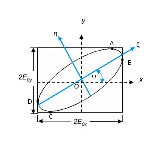
\includegraphics[width = 0.4\textwidth]{Chapter4/Figures/polellipse.eps}
 \caption{An elliptically polarized wave and the polarization ellipse.}
 \label{fig:PolEllipse}
\end{figure}
 
\begin{eqnarray}\label{eq:eq5}
\small
 	A: +E_{0x} \cos\delta,  +E_{0y} \hspace{1cm}
 	B: +E_{0x},  +E_{0y}\cos\delta \\ \nonumber
 	C: -E_{0x} \cos\delta, -E_{0y}\ \hspace{1cm}
 	D: -E_{0x},  -E_{0y}\cos\delta 	
\end{eqnarray}
\begin{equation}\label{eq:eq6}
	\textit{A} = \pi E_{0x}E_{0y}\sin\delta~.	
\end{equation}

\noindent Different values of $E_{0x}$, $E_{0y}$, and $\delta$ form various shapes of polarized ellipse and create different states of polarized light, including;

\begin{itemize}
	\item \textbf{Linearly horizontal / vertical polarized light}\\
	 When one of the transverse components does not exist ($E_{0y}$ = 0 or $E_{0x}$ = 0), oscillation happens in one direction only ($x$ or $y$ respectively).
	 The oscillation in $x$ direction is called linearly horizontal polarized and in the $y$ direction, linearly vertical polarized light.  
	\item \textbf{Linear $+45^{\circ}$ / $-45^{\circ}$ polarized light}\\
	 When $\delta = 0$ or $\pi$, Eq.~\ref{eq:eq4} is formulated by Eq. \ref{eq:eq7}.
	 In this form, light is linearly polarized with a slope of $\pm E_{0y} / E_{0x}$.
	 In this case, if $E_{0x} = E_{0y}$, the light is said to be linearly $+45^{\circ}$ polarized for parameter $\delta = \pi$ and linearly  $-45^{\circ}$ polarized for $\delta = 0$. 
	 \begin{equation}\label{eq:eq7}
	 \small
	 	E_{x} = \pm (\frac{E_{0y}}{E_{0x}})E_{y}~.
	 \end{equation}	 
	 \item \textbf{Left / right circular polarized light}\\
	When $\delta = \pi/2$ or $3\pi/2$, Eq.~\ref{eq:eq4} indicates the identical standard equation of the ellipse.
	In this condition, if $E_{0x} = E_{0y} = E_{0}$, the ellipse transforms into a circle and the light is said to be circularly left polarized ($\delta = \pi/2$) or circularly right polarized ($\delta = 3\pi/2$).
	\item \textbf{Un-polarized light}\\
	When the phase difference $\delta$ is unpredictable and rapidly varies in time, the light is said to be un-polarized.
	In this case, there is no particular polarization direction and the electrical field is equally distributed in all directions.
	 \end{itemize} 

Besides amplitudes and phase differences, a polarization ellipse contains two other elliptical parameters, the angle of rotation $\psi$ and the ellipticity angle $\chi$.
These two parameters are defined using the angle $\alpha$.
This angle is defined as $\tan(\alpha) = E_{0y}/E_{0x}$, where $\alpha$ is within the limits of $ 0\leq \alpha \leq \pi/2$.
Using this definition, the rotation and ellipticity angle of an ellipse is formulated as: 
\begin{subequations}\label{eq:eq8}
\small
	\begin{align}
	\tan 2\psi = \frac{2E_{0x}E_{0y}\cos\delta }{E_{0x}^{2}-E_{0y}^{2}} = (\tan 2\alpha) \cos\delta  \hspace{2 cm}  0\leq \psi \leq \pi~, \\
	\sin 2\chi =\frac{2E_{0x}E_{0y}\sin\delta }{E_{0x}^{2}+E_{0y}^{2}}= (\sin 2\alpha) \sin\delta  \hspace{1 cm}   -\pi/4\leq \chi\leq \pi/4~.
	\end{align}
\end{subequations}

The handedness of the elliptical polarization state can be defined using the sign $\chi$.
If $\chi$ is negative, then  $\delta$ is also negative and the field rotates counter-clockwise (from $x$ to $y$) which leads to a left handed orientated elliptical state.
On the other hand, if $\chi$ is positive, the polarization state is orientated to the right.
